%---------- Inleiding ---------------------------------------------------------

% TODO: Is dit voorstel gebaseerd op een paper van Research Methods die je
% vorig jaar hebt ingediend? Heb je daarbij eventueel samengewerkt met een
% andere student?
% Zo ja, haal dan de tekst hieronder uit commentaar en pas aan.

%\paragraph{Opmerking}

% Dit voorstel is gebaseerd op het onderzoeksvoorstel dat werd geschreven in het
% kader van het vak Research Methods dat ik (vorig/dit) academiejaar heb
% uitgewerkt (met medesturent VOORNAAM NAAM als mede-auteur).
% 

\section{Inleiding}%
\label{sec:inleiding}

Het efficiënt beheren van gegevens en bestanden wordt steeds belangrijker voor organisaties, 
inclusief kleinere organisaties zoals sportclubs. Aquarius Zwemclub Lebbeke (AZL) maakt momenteel 
gebruik van Dropbox om bestanden te delen tussen lesgevers, maar er zijn verschillende problemen. 
De toegangsrechten zijn niet altijd actueel, er is geen integratie met zowel de WordPress-website als de webapplicatie, en sommige 
lesgevers hebben geen Dropbox-account, waardoor ze geen toegang hebben tot de cloudomgeving. 
Dit leidt extra handmatig werk voor de beheerders.

Dit onderzoek richt zich op het vinden van een geschikt alternatief voor Dropbox dat beter aansluit 
bij de behoeften van AZL. Het doel is om een cloudopslagoplossing te vinden die eenvoudig te beheren is, 
die zorgt voor duidelijke en up-to-date toegangsrechten, en die goed integreert met de huidige systemen van de zwemclub. 
Dit zal het voor lesgevers makkelijker maken om toegang te krijgen tot de juiste bestanden en mappen, en tegelijkertijd de 
administratieve werklast voor de beheerders verlagen.

De centrale vraag in dit onderzoek is: \textit{Hoe kan AZL een cloudopslagoplossing implementeren die zorgt voor een beter beheer van de 
toegang tot bestanden, eenvoudig integreert met de bestaande systemen, en gebruiksvriendelijk is voor alle lesgevers, zonder dat zij hiervoor 
een extra account hoeven aan te maken?} Om deze vraag te beantwoorden, worden de volgende deelvragen onderzocht:
\begin{itemize}
    \item Wat zijn de mogelijkheden om een geschikte cloudopslagoplossing te voorzien?
    \item Wat zijn de voor- en nadelen van de verschillende oplossingen die beschikbaar zijn?
    \item Hoe kan elke mogelijke oplossing worden geïntegreerd met de bestaande systemen van AZL?
    \item Hoe kan het beheer van de toegang tot bestanden zo efficiënt en gebruiksvriendelijk mogelijk worden ingericht?
    \item Wat is de kostprijs van de verschillende oplossingen, en hoe verhoudt deze zich tot het budget van AZL?
\end{itemize}
Deze deelvragen vormen samen een gestructureerde aanpak om de centrale vraag te beantwoorden en een passende cloudopslagoplossing 
te vinden die aansluit bij de specifieke noden van de zwemclub.

Het doel van dit onderzoek is om verschillende cloudopslagoplossingen te vergelijken, de voor- en nadelen van elke oplossing te evalueren en uiteindelijk een werkend prototype (proof of concept) te ontwikkelen van de beste oplossing voor AZL. Het resultaat zal niet alleen een proof of concept bevatten, maar ook concrete aanbevelingen voor de implementatie van de gekozen oplossing.

%---------- Stand van zaken ---------------------------------------------------

\section{Literatuurstudie}%
\label{sec:literatuurstudie}

\subsection{Huidige IT-infrastructuur bij AZL}
Aquarius Zwemclub Lebbeke (AZL) maakt momenteel gebruik van een eenvoudige maar doeltreffende IT-infrastructuur:
\begin{itemize}
    \item \textbf{Hosting}: De WordPress-website en een webapplicatie gebouwd met Angular en Node.js zijn gehost op DigitalOcean.
    \item \textbf{E-mailservices}: De SMTP-server wordt gehost bij AWS, dit omdat deze functionaliteit niet beschikbaar is bij DigitalOcean.
    \item \textbf{Cloudopslag}: Voor het delen van bestanden tussen lesgevers wordt Dropbox gebruikt.
\end{itemize}
Hoewel deze infrastructuur functioneel is, kent AZL verschillende uitdagingen: er is geen integratie tussen de cloudopslag en de 
WordPress-website of webapplicatie, en geautomatiseerd toegangsbeheer ontbreekt. Een complete oplossing kan deze problemen aanpakken 
door integratie tussen de cloudopslag en de applicaties mogelijk te maken, wat zal zorgen voor een gebruiksvriendelijkere en efficiëntere werking.

%---------- Methodologie ------------------------------------------------------
\section{Methodologie}%
\label{sec:methodologie}

\subsection{Fase 1: Requirements Verzamelen}
In deze fase wordt de focus gelegd op het verzamelen van de vereisten voor een nieuwe cloudopslagoplossing voor Aquarius Zwemclub Lebbeke (AZL). Gezien de aard van de bestaande problemen met de huidige Dropbox-implementatie, wordt er voornamelijk samengewerkt met de webmaster, die verantwoordelijk is voor het beheer van de gedeelde mappen. Dit zorgt voor een gedetailleerd inzicht in de huidige knelpunten en de behoeften van de club met betrekking tot cloudopslag.

Het doel van deze fase is om zowel functionele als niet-functionele eisen in kaart te brengen voor de cloudopslagoplossing die moet worden geïntegreerd met de bestaande infrastructuur, waaronder de WordPress-website en de webapplicatie voor lesgevers (gebaseerd op Angular en Node.js). Belangrijke vraagstukken die moeten worden onderzocht zijn onder andere:
\begin{itemize}
    \item \textbf{Toegangsbeheer}: Hoe kan toegang tot de cloudopslag op een efficiënte en veilige manier worden geregeld voor de verschillende lesgevers? Er moet worden nagedacht over wie toegang krijgt en hoe dit dynamisch kan worden aangepast naargelang de status van de lesgevers (bijvoorbeeld wanneer zij stoppen of tijdelijk geen toegang nodig hebben).
    \item \textbf{Beveiliging en privacy}: Hoe kunnen we ervoor zorgen dat lesgevers enkel toegang hebben tot de bestanden en mappen die voor hen relevant zijn, zonder dat andere informatie toegankelijk is?
    \item \textbf{Integratie met bestaande systemen}: Kan de nieuwe oplossing naadloos worden geïntegreerd met de bestaande webapplicatie voor lesgevers en de publieke website van de zwemclub? Dit omvat zowel technische integratie als gebruikersgemak.
    \item \textbf{Kosten}: Wat zijn de kosten van de nieuwe oplossing en hoe verhouden deze zich tot de huidige Dropbox-oplossing? Dit kan de keuze voor bepaalde cloudopslagoplossingen beïnvloeden.
    \item \textbf{Beheer en onderhoud}: Hoe kan de oplossing eenvoudig worden beheerd door de webmaster en andere betrokkenen, en welke ondersteuning is nodig om te zorgen voor een duurzame implementatie?
\end{itemize}

Tijdens deze fase zal ook de MoSCoW-methode worden toegepast om de prioriteiten te bepalen, waarbij de belangrijkste vereisten worden gemarkeerd als ‘Must Have’, gevolgd door ‘Should Have’, ‘Could Have’, en ‘Won’t Have’. Het resultaat van deze fase zal een gedetailleerde lijst van vereisten zijn, inclusief prioriteitstelling, die als basis zal dienen voor de verdere ontwikkeling van de cloudopslagoplossing.

\subsection{Fase 2: Long List van Mogelijke Cloudoplossingen}
In deze fase wordt een uitgebreide lijst van mogelijke technologische oplossingen en alternatieven (long list) opgesteld. Dit gebeurt door middel van een literatuuronderzoek en het verkennen van bestaande software en systemen voor cloudopslag en documentbeheer die voldoen aan de specifieke behoeften van Aquarius Zwemclub Lebbeke (AZL). Het doel is om een breed scala aan mogelijke oplossingen te onderzoeken, waarbij geen alternatieven worden uitgesloten, zodat alle opties overwogen kunnen worden.

AZL gebruikt op dit moment Dropbox voor gedeelde mappen, maar dit brengt diverse problemen met zich mee. Zo vergeten lesgevers vaak dat deze mappen bestaan, hebben niet de juiste rechten, of kunnen er niet bij zonder Dropbox-account. Om deze redenen richt dit onderzoek zich op het vinden van alternatieve cloudoplossingen die eenvoudig geïntegreerd kunnen worden met AZL’s bestaande webapplicatie voor lesgevers (ontwikkeld in Angular en Node.js) of de publieke WordPress-website. Belangrijke selectiecriteria zijn onder andere gebruiksvriendelijkheid, efficiënt toegangsbeheer, beveiligingsopties en kosteneffectiviteit.
\subsection{Fase 3: Short List}
In deze fase wordt een selectie gemaakt uit de eerder opgestelde longlist met mogelijke technologische oplossingen. De selectie gebeurt op basis van een vergelijkende analyse waarin de alternatieven worden beoordeeld aan de hand van de criteria opgesteld in fase 1, zoals efficiënt toegangsbeheer, integratie met de bestaande webapplicatie en de WordPress-website, beveiliging en kosten. Een samenvattende tabel vat de voor- en nadelen van elk alternatief samen, wat helpt om de systemen te identificeren die het beste aansluiten bij de specifieke behoeften van AZL. De alternatieven die het meest veelbelovend zijn op het gebied van functionaliteit, veiligheid en kostenbesparing worden geselecteerd voor verder onderzoek in de volgende fase.
\subsection{Fase 4: Proof of Concept (PoC)}
In deze fase wordt een Proof of Concept (PoC) ontwikkeld om te testen of de geselecteerde oplossing daadwerkelijk in staat is de huidige problemen binnen AZL op te lossen. De PoC bestaat uit een werkend prototype van de cloudopslagoplossing, dat als feature wordt geïntegreerd in de bestaande webapp. Na het maken van de PoC wordt deze getest door de webmaster en enkele lesgevers om te controleren of de oplossing voldoet aan de gestelde eisen en verwachtingen. De feedback van de gebruikers wordt verzameld en geanalyseerd om eventuele verbeteringen aan te brengen in de PoC. Het doel van deze fase is om te valideren of de geselecteerde oplossing daadwerkelijk een verbetering is ten opzichte van de huidige Dropbox-implementatie en om te bepalen het onderzochte alternatief daadwerkelijk geschikt is voor implementatie binnen AZL.
\subsection{Fase 5: Evaluatie en Conclusies}
Na de implementatie van het Proof of Concept volgt een grondige evaluatie van de resultaten. De focus ligt op de effectiviteit van de oplossing en in hoeverre deze de problemen rondom het documentbeheer en toegangsbeheer van AZL oplost. Eventuele tekortkomingen of beperkingen worden gedocumenteerd, en verbeterpunten worden geïdentificeerd om de oplossing verder te optimaliseren. Ook wordt de impact van de gekozen oplossing op de dagelijkse werking van AZL geëvalueerd, zoals de tijdsbesparing, het gebruiksgemak voor lesgevers en de verbeterde toegang tot informatie.

Op basis van de evaluatie worden conclusies getrokken en aanbevelingen gedaan voor de implementatie van de oplossing binnen AZL.
\subsection{Visualisatie en Tijdsplanning}

\begin{figure}[h!]
    \centering
    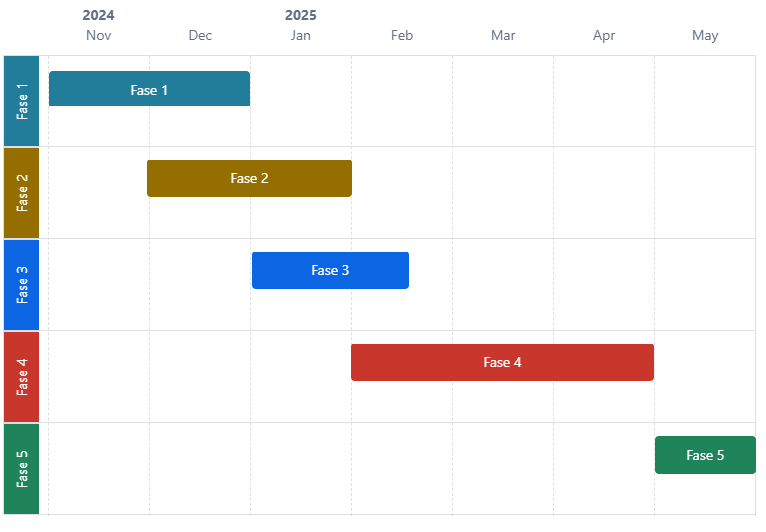
\includegraphics[width=.5\textwidth]{../graphics/Chart-Tijd-Visualisatie.png}
    \caption{Tijdsplanning van het project}
    \label{fig:tijdsplanning}
\end{figure}


%---------- Verwachte resultaten ----------------------------------------------
\section{Verwacht resultaat, conclusie}%
\label{sec:verwachte_resultaten}

De meerwaarde van deze bachelorproef voor de doelgroep, de Aquarius Zwemclub Lebbeke, is duidelijk: de implementatie van een robuuste cloudopslagoplossing zal niet alleen de werkprocessen voor de lesgevers verbeteren, maar ook de algehele efficiëntie van de club vergroten. Door de administratieve processen te automatiseren en beter beheersbaar te maken, wordt er tijdswinst geboekt, wat meer ruimte biedt voor de daadwerkelijke activiteiten van de club. Bovendien zal de verbetering van de toegang en beveiliging van documenten bijdragen aan een professionelere werking van de zwemclub.

De verwachte conclusie van deze bachelorproef is dan ook dat het gekozen cloudopslagsysteem zowel technisch haalbaar als praktisch effectief zal zijn voor de behoeften van de zwemclub. Mocht de gekozen oplossing echter niet voldoen aan de verwachtingen, dan zal het onderzoek zich richten op het identificeren van de tekortkomingen en de redenen waarom deze oplossing niet geschikt bleek. In dat geval zal er verder onderzocht worden welke alternatieven nog beter aansluiten bij de eisen van AZL.